\section{Requirement Specifications}
\begin{frame}{Requirement Specifications}{\textit{Grundfos} Case}
\begin{itemize}
    \item Industrial manipulator
    \item Stationary impeller
    \item Cycle time - within $45.0$ $s$
    \item Robot cell - less than $4\cdot10^{3}$ $\times$ $4\cdot10^{3}$ $mm$
\end{itemize}
\vspace{5mm}
\centering{

\includegraphics[width=0.7\textwidth]{graphics/andrej/grundfos_logo}

\tiny{(grundfos.com)}}
\end{frame}

\begin{frame}{Requirement Specifications}{Processing Tool}
\begin{columns}
\column{0.55\textwidth}
\begin{itemize}
    \item \textit{HIGHYAG BIMO W}
        \begin{itemize}
            \item Fibre laser processing head
            \item $6.00\cdot10^{3}$ $W$
            \item $4.40$ $kg$
            \item $479 \times 90.0 \times 388$ $mm$
            % \item Onboard camera
        \end{itemize}   
\end{itemize}
\column{0.45\textwidth}
\centering
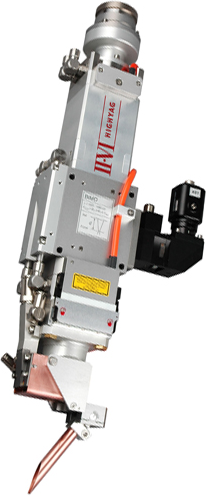
\includegraphics[width=.65\textwidth]{graphics/andrej/bimo}

\tiny{(highyag.com)}
\end{columns}
\end{frame}

%Hello there, I am sorry for the intrusion and interruption, kind sir, but I was hoping you could help me out with a slight problem I am experiencing. You see, I wish to insert a table, where each row is of interchanging colors, I am able to do so, even with the colors that I wish to use, however, due to my lack of experience in the area, I cannot do it in a proper manor. So far, I am inserting "\definecolor{colorK}{HTML}{DEDEDE}" just before I use it, with no problems. I do however wish to insert it, so that it affects the entire file. I believe the proper way is to insert it somewhere like in the "aausidebartheme" and in the preamble insert "\userpackage{color}", but I would require assistance in this. 

% \begin{frame}{Requirement Specifications}{Design and Performance Requirements}
%     \centering
%     \resizebox{\textwidth}{!}{
%     \begin{tabular}{l}
%     \hline
%     \rowcolor{beamer@headercolor} \multicolumn{1}{c}{\color{white}{Design Requirements}} \\
%     \hline
%     Dimensions of the workcell must be at most $4\cdot10^{3}$ $\times$ $4\cdot10^{3}$ $mm$\\
%     \rowcolor{beamer@barcolor} Workcell safety must meet \textit{ISO} standards\\   
%     Workspace must be equipped with a suitable industrial manipulator\\
%     \rowcolor{beamer@barcolor} Material flow must happen without human aid\\
%     Sub-components must be held in a fixed position\\
%     \hline
%     \end{tabular}}

% \vspace{5mm}

%     \resizebox{\textwidth}{!}{
%     \begin{tabular}{l}
%     \hline
%     \rowcolor{beamer@headercolor} \multicolumn{1}{c}{\color{white}{Performance Requirements}} \\
%     \hline
%     Cycle time must be no more than $45.0$ $s$\\
%     \rowcolor{beamer@barcolor} Welding velocity must be kept constant at $167$ $mm/s$\\
%     Relative distance must be constant at $480$ $mm$\\
%     \rowcolor{beamer@barcolor} The industrial manipulator must have at least five degrees of freedom\\
%     Relative angle must be perpendicular during vane welding\\
%     \rowcolor{beamer@barcolor} Relative angle during hub welding must be $30.0\degree$\\
%     Deviation must not exceed $0.300$ $mm$\\
%     \hline
%     \end{tabular}}
%     \centering
% \end{frame}



\begin{frame}{Requirement Specifications}{Design and Performance Requirements}
    \centering

    \begin{tabular}{m{3.475cm}m{3.175cm}}
    \hline \rowcolor{table_first_row} \multicolumn{2}{c}{\cellcolor{beamer@normaltextcolor} {\color{white} Design Requirements}} \\ \hline
    Workcell &  $\leq$ $4\cdot10^{3}$ $\times$ $4\cdot10^{3}$ $mm$ \\
    \rowcolor{beamer@barcolor} Safety & \textit{ISO} Standards \\
    Industrial Manipulator  & Suitable for Welding\\ 
    \rowcolor{beamer@barcolor} Material Flow &  Autonomous \\
    Sub-Components &  Fixed \\ \hline
    \end{tabular}

\vspace{5mm}

    \begin{tabular}{m{3.475cm}m{3.175cm}} 
    \hline \rowcolor{table_first_row} \multicolumn{2}{c}{\cellcolor{beamer@normaltextcolor} {\color{white} Performance Requirements}} \\ \hline
    Cycle Time &  $\leq$ $45.0$ $s$ \\ 
    \rowcolor{beamer@barcolor} Constant Velocity &  $167$ $mm/s$ \\
    Relative Distance & $480$ $mm$ \\ 
    \rowcolor{beamer@barcolor} Relative Angle - Vanes &$90.0$ $\degree$ \\
    Relative Angle - Hub &  $30.0$ $\degree$ \\ 
    \rowcolor{beamer@barcolor} Degree of Freedom &  $\geq$ $5$ \\
    Deviation & $\leq$ $0.300$ $mm$\\ \hline
    \end{tabular}
    
    % \centering\arraybackslash 
    
\end{frame}